\documentclass[12pt]{article}
\usepackage[margin=1.0in]{geometry} %page layout
\usepackage[usenames,dvipsnames]{color} %color
\definecolor{light-gray}{gray}{0.95}
\definecolor{darkgreen}{rgb}{0,0.4,0}
\usepackage{graphicx, subfigure} %figures
\usepackage{url, hyperref} %cross-referencing
\usepackage{amsmath, amssymb} %math
\usepackage{listings} %source code
\lstset{breaklines=true,
breakindent=0pt,
prebreak=\mbox{\tiny$\searrow$},
postbreak=\mbox{{\color{blue}\tiny$\rightarrow$}},
numbers=left,
commentstyle=\color{darkgreen},
numberblanklines=false,
frame=single,
captionpos=b,
backgroundcolor=\color{light-gray}}
\usepackage[3D]{movie15} %for movies (needs hyperref)
	\newenvironment{changemargin}[2]
	{
	  	\begin{list}{}
		{
			\setlength{\topsep}{0pt}%
			\setlength{\leftmargin}{#1}%
			\setlength{\rightmargin}{#2}%
			\setlength{\listparindent}{\parindent}%
			\setlength{\itemindent}{\parindent}%
			\setlength{\parsep}{\parskip}%
		}
	  	\item[]
		}
		{\end{list}
	}
\author{Salman Aslam\\Georgia Tech}
\title{RVQ tracking}
\author{Salman Aslam\\ Georgia Institute of Technology}
\date{}
\definecolor{darkgreen}{rgb}{0,0.5,0}
\newcommand{\Ntrg}{\big[N_{t=1, m=1} + \lambda \big] + \big[N_{t=1, m=2} + \lambda \big] + \ldots + \big[N_{t=1, m=M} + \lambda \big]}
\newcommand{\jointcnt}{\sum\limits_{n_{trg}=1}^{N_{trg}}I(X_t=x_t, X_{t-1}=x_{t-1})}
\newcommand{\singlecnt}{\sum\limits_{n_{trg}=1}^{N_{trg}}I(X_{t-1}=x_{t-1})}
\newcommand{\singlep}{p(X_{t-1}=x_{t-1})}
\newcommand{\singlepone}{p(X_{t-1}=1)}
\newcommand{\singleptwo}{p(X_{t-1}=2)}
\newcommand{\singlepM}{p(X_{t-1}=M)}
\newcommand{\condp}{p(X_t=x_t | X_{t-1}=x_{t-1})}
\newcommand{\jointp}{p(X_t=x_t, X_{t-1}=x_{t-1})}
\newcommand{\KmeansOuterSum}{\sum\limits_{k=1}^K}
\newcommand{\KmeansInnerSum}{\sum\limits_{{i=1 \atop x_i \in \mathcal{K}_k}}^N}
\newcommand{\KmeansSum}{\KmeansOuterSum \KmeansInnerSum}
\newcommand{\RVQInnerSum}{\sum\limits_{{i=1 \atop g_i \mapsto m_{\tau, s}}}^N}
\newcommand{\RVQOuterSum}{\sum_{s=1}^S}
\newcommand{\RVQsum}{\KmeansOuterSum \sum\limits_{{i=1 \atop g_i \in \mathcal{K}_k}}^N}
\newcommand{\KmeansInner}{{(x_i - \mu_k)}^2}
\newcommand{\RVQinner}{            {(x_i  - \hat{\mu}^{(k)})}^2}
\newcommand{\RVQinneralternate}{{(g_i - m_\tau^{(k)})}^2}
\newcommand{\RVQinneralternatealternate}{{(g_i - m_{\tau, s})}^2}
\newcommand{\KmeansError}{\KmeansSum \KmeansInner}
\newcommand{\RVQerror}     {\KmeansSum \RVQinner}
\newcommand{\RVQerroralternate}{\RVQsum \RVQinneralternate}
\newcommand{\RVQunit}{x_i -\bigg(\sum_{t=1}^Tm^{(k)}_t\bigg)}
\newcommand{\RVQequivalentCodevector}{\sum_{t=1 }^Tm^{(k)}_t}
\newcommand{\RVQequivalentCodevectorBroken}{\sum_{t=1 \atop t \neq \tau}^Tm^{(k)}_t+ m^{(k)}_\tau}
\newcommand{\RVQmultipleKmeans}{x_i -\bigg(\RVQequivalentCodevectorBroken\bigg)}
\newcommand{\RVQmultipleKmeansone}{x_i -\sum_{t=2}^Tm^{(k)}_t+ m^{(k)}_1\bigg)}
\newcommand{\RVQmultipleKmeansonealternate}{\bigg(x_i -\sum_{t=1 \atop t \neq \tau}^Tm^{(k)}_t\bigg) - m^{(k)}_\tau}
\newcommand{\RVQmultipleKmeanstwo}{x_i -\bigg(\sum_{t=1 \atop t \neq 2}^Tm^{(k)}_t+ m^{(k)}_2\bigg)}
\newcommand{\RVQmultipleKmeansT}{x_i -\bigg(\sum_{t=1}^{T-1}m^{(k)}_t+ m^{(k)}_2\bigg)}
\newcommand{\EucMatrix}
{
\left[
\begin{array}{lll}
r_{11} & r_{12} & t_x \\ 
r_{21} & r_{22} & t_y \\ 
0 & 0 & 1 \\ 
\end{array}
\right]
}	

\newcommand{\SimMatrix}
{
\left[
\begin{array}{lll}
sr_{11} & sr_{12} & t_x \\ 
sr_{21} & sr_{22} & t_y \\
0 & 0 & 1 \\ 
\end{array}
\right]
}

\newcommand{\AffMatrix}
{
\left[
\begin{array}{lll}
a &b & t_x \\ 
c & d & t_y \\
0 & 0 & 1 \\
\end{array}
\right]
}

\newcommand{\ProjMatrix}
{
\left[
\begin{array}{lll}
h_{11} & h_{12} & h_{13} \\ 
h_{21} & h_{22} & h_{23} \\ 
h_{31} & h_{32} & h_{33} \\ 
\end{array}
\right]
}

\newcommand{\RotMatrixTheta}
{
\left[
\begin{array}{rr}
\cos(\theta) & -\sin(\theta) \\ 
\sin(\theta) & \cos(\theta) \\ 
\end{array}
\right]
}

\newcommand{\RotMatrixPhi}
{
\left[
\begin{array}{rr}
\cos(\phi) & -\sin(\phi) \\ 
\sin(\phi) & \cos(\phi) \\ 
\end{array}
\right]
}

\newcommand{\RotMatrixminusPhi}
{
\left[
\begin{array}{rr}
\cos(-\phi) & -\sin(-\phi) \\ 
\sin(-\phi) & \cos(-\phi) \\ 
\end{array}
\right]
}


\newcommand{\EigenvalueMatrix}
{
\left[
\begin{array}{cc}
\lambda_1 & 0\\
0 & \lambda_2
\end{array}
\right]
}

\newcommand{\bigMatrix}
{
s \left[
\begin{array}{cc}
 (r)(a) + b &  (r)(d) - c \\
 (r)(c) - d &  (r)(b) + a
\end{array}
\right]
}


\newcommand{\bigMatrixTwo}
{
\left[
\begin{array}{cc}
(\lambda_2) p + (\lambda_1) q & (\lambda_2) s  - (\lambda_1) r \\
(\lambda_2) r  - (\lambda_1) s & (\lambda_2) q + (\lambda_1) p
\end{array}
\right]
}
\newcommand{\dr}{(\mathbf{x}_i-\boldsymbol\mu_k)^T(\mathbf{x}_i-\boldsymbol\mu_k) + \lambda({Q_{\textrm{max}}-Q_i})}

\begin{document}
\maketitle
\rule[0pt]{\textwidth}{1pt}
\tableofcontents
\rule[0pt]{\textwidth}{1pt}
\newcommand{\dr}{(\mathbf{x}_i-\boldsymbol\mu_k)^T(\mathbf{x}_i-\boldsymbol\mu_k) + \lambda({Q_{\textrm{max}}-Q_i})}

\begin{abstract}
A learning-based tracking framework builds the target model while it tracks, thus avoiding the costly step of building target models prior to tracking.  This has been demonstrated successfully for PCA based tracking using publicly-available challenging datasets.  In this work, we use Residual Vector Quantization in a learning-based tracking framework using the same datasets and show that RVQ performs as well as PCA.  Moreover, we introduce 2 new distance metrics for relative weighting of target candidates allowing RVQ to be used as a generative model, similar to the way probabilistic PCA converts PCA into a generative framework.
\end{abstract}

%================================
\section{Introduction}
%================================
Visual tracking is the task of estimating a target's state over time.  In many cases, the state represents target position and a bounding box around it, or its contour.  However, this is a challenging problem due to the following reasons:

\begin{enumerate}
\item \underline{Appearance and contour changes}:  A target of interest can undergo arbitrary change in appearance and contour.  This can be due to the following reasons:
\begin{enumerate}
\item \underline{Pose change}:  The target can rotate and present a different view to the camera.
\item \underline{Warping}: The target can undergo warps, such as expression changes for humans.
\item \underline{Self occlusion}:  The target can be occluded or unoccluded by itself or its surroundings.
\item \underline{Blur}:  Motion blur can severely distort a target's appearance.
\item \underline{Structured noise}:  The target can change appearance in an orderly manner, for instance, a target of interest can put on or remove glasses or a hat.
\item \underline{Random noise}:  Random noise is added to the light rays coming from a target of interest.  On the hardware side, this is caused by atmospheric effects in the optical channel.  On the receiving side, it is caused by sensor noise, electronics noise and EMI (electromagnetic interference).  On the software side, it can be caused by compression artefacts.
\item \underline{Non-symmetic BRDF}:  The light reflected off of an object in all directions is modeled by the BRDF (Bidirectional Radiation Transfer Function).  Since this function may not be symmetric in all directions, the amount of light reflecting off of the object may be different in different directions.  Multiple cameras viewing the same point will receive different intensity levels.
\end{enumerate}
\item \underline{Lighting change}: Lighting changes can be caused by turning on or off lights in indoor environments, or moving into or out of shades in outdoor environments.
\item \underline{Sudden motion (target or camera)}:  Besides motion blur, sudden motion by the target or camera can cause the target to exit the window in which the tracker looks for the target leading to incorrect track assignment.
\end{enumerate}

								\begin{figure}
								\centering
								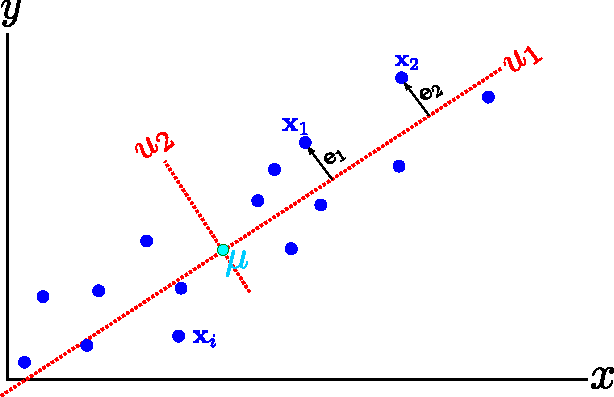
\includegraphics[width=0.45\textwidth]{figs/PRML_PCA_problem.pdf}
								\caption{In $\mathbb{R}^2$, a reduced eigenspace means that eigenvector $u_2$ is discarded.  Vectors $\mathbf{x}_1$ and $\mathbf{x}_2$ have the same projection error on eigenvector $u_1$ even though $\mathbf{x}_1$ is closer to the mean $\boldsymbol\mu$ of the training data $\mathbf{x}_i$.}
								\label{fig:PRML_PCA_problem}
								\end{figure}

For a tracker that tries to learn the appearance and/or contour model of the target, inclusion of background pixels is an added problem that can cause drift.  If none of the problems mentioned above were present, a simple template matching stategy would suffice for robust tracking.  This has complexity $O(nm)$, where $n$ is the number of pixels in the target and $m$ is the number of locations at which the target is searched.  For most practical situations, this does not represent significant computational load and can be done in real time even while tracking several targets.

In this work, we try to address single-target visual-tracking under several of the challenges mentioned above while trying to learn the appearance model of the target.  Seminal work here can be traced back to 1996 when Black and Jepson experimented with tracking using an eigenspace representation of the target appearance model~\cite{1998_JNL_Eigentracking_Black}.  The next notable work is by Moghaddam and Pentland, 1997~\cite{1997_JNL_EigenTRK_Moghaddam} in which they try to address a fundamental limitation of PCA.  In PCA, 2 vectors, $\mathbf{x}_1$ and $\mathbf{x}_2$ can have the same distance to a reduced eigenspace even if they have different distance to the mean of the data.  This is shown for a trivial case in $\mathbb{R}^2$ in Figure~\ref{fig:PRML_PCA_problem} where $\mathbf{e}_1=\mathbf{e}_2=\mathbf{e}$ even though $\mathbf{x}_1$ is closer to the mean $\boldsymbol\mu$ than $\mathbf{x}_2$.  They formulate the problem using DIFS (distance in feature space) and DFFS (distance from feature space) so that both projection error and distance to the mean of the data are used while trying to determine how well the subspace explains a new data-point.  The next breakthrough came with the work of Bishop and Tipping in 1999~\cite{1999_JNL_PPCA_Tipping} where they show that a probabilistic variation of PCA (PPCA) allows PCA to be used as a generative model.  The advantage in tracking is that this methodology allows an assignment of probabilities to new data-points.  This relative weighting can be used to determine best candidates.  All three works were combined into a tracking framework for the first time by Ross et. al. in 2008~\cite{2008_JNL_subspaceTRK_Ross}.  Moreover, they used incremental SVD to make their tracker run in real time.  

								\begin{figure}[t]
								\centering
								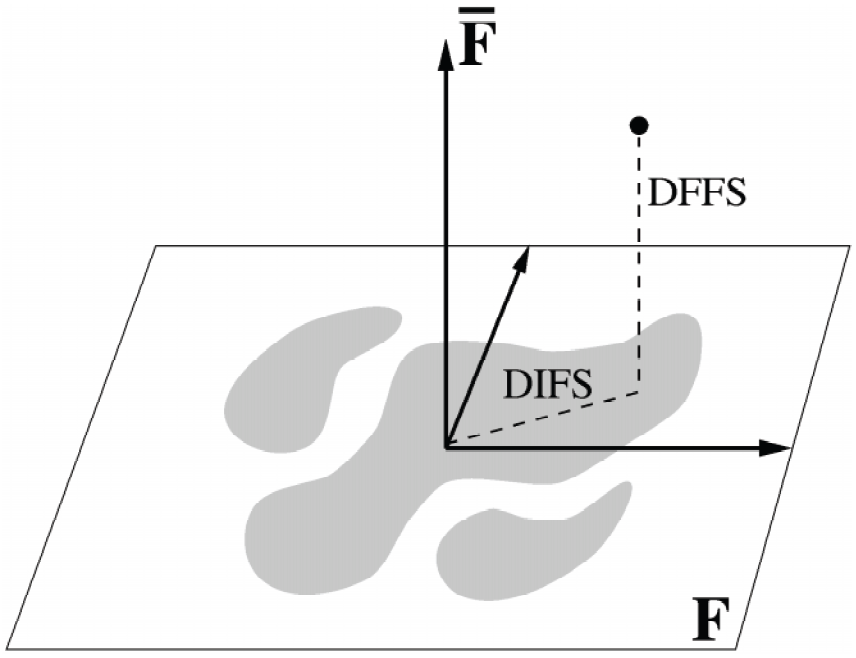
\includegraphics[width=0.5\textwidth]{figs/1998_JNL_ProbVisLearning_Moghaddam_fig3.png}
								\caption{Graphical illustration of DFFS (distance-from-feature-space) and DIFS (distance-in-feature-space).  The feature space is $\mathbf{F}$ while the subspace orthogonal to the feature space is $\bar{\mathbf{F}}$.  DFFS is the signal residual error and DIFS is the $\mathbf{F}$-space likelihood \cite{1997_JNL_EigenTRK_Moghaddam}.}
								\label{fig:1997_JNL_DIFSDFFS_Moghaddam}
								\end{figure}

Here, we extend this work using RVQ instead of PCA and introducing two new distance based measures for relative weighting of tracking candidates.  The result is a generative framework for RVQ that leads to robust tracking.  Whereas RVQ was first introduced by Juang and Gray in 1982~\cite{1982_CNF_SpeechRVQ_JuangGray}, subsequently greatly extended by the seminal work of Barnes~\cite{1991_CNF_DesignPerformanceRVQ_Frost,1992_JNL_RVQ_Barnes,1992_CNF_ImageCodingRVQ_Kossentini,1993_sigmaTrees_Barnes,1993_JNL_RVQDSC_Barnes,1995_JNL_OptimalityRVQ_Kossentini,1996_CNF_VQclassification_Barnes,1996_JNL_AdvancesRVQ_Barnes,2002_JNL_SigmaTrees_Barnes,2004_CNF_DSSAdataMining_Barnes,2007_JNL_Katrina_Barnes,2007_JNL_IDDM_Barnes} and widely known in the signal processing and information theory communities, relatively little attention has been given to this work in the computer vision and machine learning fields where a much simpler version, K-means, has been widely used.  Our goal is to remedy this situation and introduce RVQ in the context of an important and challenging problem, visual target tracking.


%================================
\section{Theory}
%================================
It has been shown by Roweis and Ghahramani~\cite{1999_JNL_Gaussian_roweis} that under the assumption of gaussian noise, factor analysis (FA), principal component analysis (PCA), mixtures of gaussian (MoG) clusters, vector quantization (VQ), independent components analysis (ICA), Kalman filters and hidden Markov models (HMMs) are instances of a single basic generative model, the linear gaussian model.  The linear gaussian model can be written as,

\begin{equation}
\begin{array}{llllllllllllll}
\mathbf{x}_{t+1} &=  \mathbf{A}\mathbf{x}_{t} +  \mathbf{w}_t   & & & \mathbf{w}_t \sim \mathcal{N}(0, \mathbf{Q})\\
\mathbf{y}_t 		 &=  \mathbf{C}\mathbf{x}_{t} +  \mathbf{v}_t    & & & \mathbf{v}_t \sim \mathcal{N}(0, \mathbf{R})
\end{array}
\label{LGM}
\end{equation}

where $\mathbf{A}$ is the state transition matrix, $\mathbf{C}$ is the observation matrix, and $\mathbf{w}_t$ and $\mathbf{v}_t$ are zero-mean gaussian random variables.  Under conditions where each data point $\mathbf{x}$ was generated independently and identically without any temporal ordering, i.e., $\mathbf{A}=\mathbf{0}$, we can write,

\begin{equation}
\begin{array}{llllllllllllll}
\mathbf{x} &= \mathbf{w} 											& & & \mathbf{w} &\sim \mathcal{N}(0, \mathbf{Q})\\
\mathbf{y} &=  \mathbf{C}\mathbf{x} +  \mathbf{v} 		& & & \mathbf{v} & \sim \mathcal{N}(0, \mathbf{R})
\end{array}
\label{LGM1}
\end{equation}



\begin{table}[t]
\centering
\begin{tabular}{| c | c | c | c | c |}\hline
 				 	&\textbf{A}	 	&	\textbf{C}  									& \textbf{Q} 	&  \textbf{R}                                                                		\\\hline
\textbf{PCA} 	&\textbf{0}		&	principal eigenvectors of $\boldsymbol\Sigma$	& \textbf{I}  	&  $\lim\limits_{\sigma^2 \rightarrow 0} \sigma^2\mathbf{I}$ 	\\\hline
\textbf{PPCA} &\textbf{0}		& 	scaled principal eigenvectors of $\boldsymbol\Sigma$	& \textbf{I}	&										      $\sigma^2 \mathbf{I}$	 \\\hline
\textbf{FA}   	&\textbf{0}		&													& \textbf{I} 	&  diagonal matrix 																\\\hline
\textbf{VQ}	 	&\textbf{0} 	&	cluster means								& \textbf{I}	& 	-																					\\\hline
\end{tabular}
\caption{Unifying PCA, PPCA, FA, and VQ using linear gaussian models~\cite{1999_JNL_Gaussian_roweis, 1999_JNL_PPCA_Tipping}.}
\label{table:LGM_unifying}
\end{table}

Moreover, for non-linear mappings, such as in MoG and VQ, a function $\mathbf{WTA[.]}$, \emph{winner-take-all} is introduced which returns a vector with unity in one position and all remaining zeros,

\begin{equation}
\begin{array}{llllllllllllll}
\mathbf{x} &= \mathbf{WTA}(\mathbf{w}) 						& & & \mathbf{w} &\sim \mathcal{N}(\mathbf{\boldsymbol\mu}, \mathbf{Q})\\
\mathbf{y} &=  \mathbf{C}\mathbf{x} +  \mathbf{v} 		& & & \mathbf{v} & \sim \mathcal{N}(0, \mathbf{R})
\end{array}
\label{LGM2}
\end{equation}

The values for \textbf{A}, \textbf{C}, \textbf{Q} and \textbf{R} under this elegant, unifying generative framework for various algorithms, including PCA and VQ, are given in Table~\ref{table:LGM_unifying}.  Besides being inherently satisfying, this framework allows the computation of data likelihoods in the case of PCA and VQ since they both do not define a proper density in the observation space~\cite{1999_JNL_Gaussian_roweis}.  We start with likelihoods under PCA, PPCA and VQ.  Our contribution is extending this work to compute likelihoods under RVQ.

\subsection{Likelihood for PCA}
%-----------------------------------------
In a gaussian distribution, the probability of a data point $\mathbf{x}$ in $\mathbb{R}^D$ depends on the Mahalanobis distance $d$.  The output of PCA, zero-centered $\mathbf{\tilde{y}}$ is decorrelated with variances along each dimension equal to the eigenvalues $\lambda_i$ of the covariance matrix $\boldsymbol\Sigma$,


\begin{equation}
\begin{array}{lllllll}
d &= (\mathbf{x}-\boldsymbol\mu)^T\boldsymbol\Sigma^{-1}(\mathbf{x}-\boldsymbol\mu)\\
&=\mathbf{\tilde{x}}^T\boldsymbol\Sigma^{-1}\mathbf{\tilde{x}}\\
&=\mathbf{\tilde{x}}^T(\mathbf{U}\boldsymbol\Lambda\mathbf{U}^T)^{-1}\mathbf{\tilde{x}}\\
&=\mathbf{\tilde{x}}^T(\mathbf{U}\boldsymbol\Lambda^{-1}\mathbf{U}^{-1})\mathbf{\tilde{x}}\\
&=(\mathbf{U}^T\mathbf{\tilde{x}})^T\boldsymbol\Lambda^{-1}(\mathbf{U}^T\mathbf{\tilde{x}})	\\
&=\mathbf{\tilde{y}}^T\boldsymbol\Lambda^{-1}\mathbf{\tilde{y}}\\
&=\sum\limits_{d=1}^D \frac{\tilde{y}_i}{\lambda_i}\\
&=\sum\limits_{d=1}^Q \frac{\tilde{y}_i^2}{\lambda_i} + {\color{red}\sum\limits_{d=Q+1}^D} \frac{{\color{red}\tilde{y}_i^2}}{\lambda_i}, \ \ \  & \bigg(\textrm{DFFS = recon. error}={\color{red}\sum\limits_{i=1}^D e_i^2} = \sum\limits_{i=1}^D \tilde{x}_i^2 - \sum\limits_{i=1}^Q \tilde{y}_i^2= {\color{red}\sum\limits_{d=Q+1}^D} {\color{red}\tilde{y}_i^2}\bigg)\\
&=\sum\limits_{d=1}^Q \frac{\tilde{y}_i^2}{\lambda_i} + \frac{1}{\rho} {\color{red}\sum\limits_{i=1}^D e_i^2} \ \ \ & \bigg(\rho^* = \frac{1}{D-q}\sum\limits_{i=q+1}^D \lambda_i\bigg)\\
\end{array}
\label{Eqn:MoghaddamLikelihood}
\end{equation}

This formulation, first presented in~\cite{1997_JNL_EigenTRK_Moghaddam} shows that the first term in the sum is the DIFS term in Figure~\ref{fig:1997_JNL_DIFSDFFS_Moghaddam} while the second term corresponds to DFFS.  With this formulation, PCA can be used in a probabilistic framework since the error of a test vector $\mathbf{x}$ now also depends on its distance from the mean of the data.

\subsection{Likelihood for PPCA}
%-----------------------------------------
For PCA, using Equation~\ref{LGM1} and Table~\ref{table:LGM_unifying}, we have the likelihood of observing $\mathbf{y}$ given by,

\begin{equation}
p(\mathbf{y}) \sim \mathcal{N}(\boldsymbol\mu, \mathbf{C}\mathbf{C}^T + \sigma^2 \mathbf{I})
\end{equation}

Bishop and Tipping~\cite{1999_JNL_PPCA_Tipping} show that this can be done in closed form using PPCA with the following solution,

\begin{equation}
\begin{array}{lllll}
\mathbf{\boldsymbol\mu}_{\textrm{ML}} &=\frac{1}{N}\sum\limits_{i=1}^N \mathbf{x}_i\\
\sigma^2_{\textrm{ML}} &= \frac{1}{D-q}\sum\limits_{i=q+1}^D \lambda_i\\
\mathbf{C}_{\textrm{ML}} &= \mathbf{U}_q(\mathbf{\Lambda}_q - \sigma^2\mathbf{I})^{1/2} \\
\end{array}
\label{Eqn:PPCA}
\end{equation}

where, $\boldsymbol\Sigma = \mathbf{U}\mathbf{\Lambda}\mathbf{V}^T$, $\mathbf{U}_q$ are the first $q$ eigenvectors in $\mathbf{U}$, $\mathbf{\Lambda}_q$ contains the corresponding eigenvalues, $\lambda_1, \lambda_2, \ldots \lambda_q$, $D$ is the dimensionality of the data and $N$ is the number of data points.  Note that in the above equation, we have omitted multiplication with an arbitrary rotation matrix since it can be taken to be $\mathbf{I}$ without loss of generality.  

In Equation~\ref{Eqn:PPCA}, $\sigma^2_{\textrm{ML}}$ is the average variance in the discarded dimensions and $\mathbf{C}_{\textrm{ML}}$ maps $\mathbf{x}$ onto its principal components to give output $\mathbf{y}$.

								\begin{figure}[t]
								\centering
								\subfigure[Codebook and decode path taken through the RVQ~$\sigma$-tree by all 4 methods to decode the number 8.  Notice that monR is the only method unable to correctly decode.]{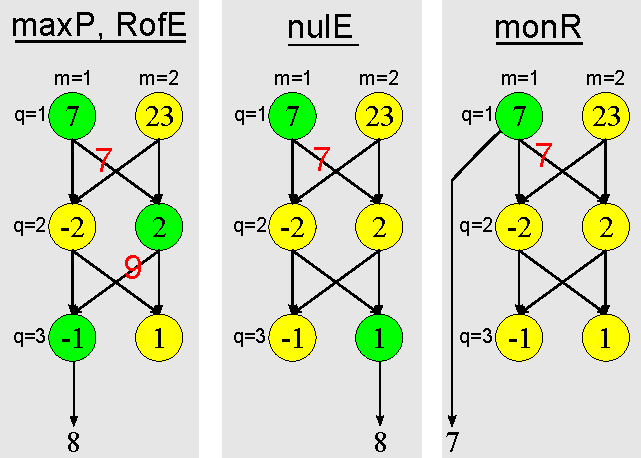
\includegraphics[height=2in]{figs/RVQ_CAC_toyExample_3x2.pdf}}
								\subfigure[Decoded outputs produced by monR.  Whereas maxP, RofE, nulE produce perfect reconstructions, monR incorrectly decodes 6, 8, 23 and 24.]{\includegraphics[height=2in]{figs/RVQ_CAC_toyExample_3x2_monR.pdf}}
								\caption{3x2 (3 stages, 2 code-vectors per stage) RVQ codebook generated with the training set, S=$\{4, 6, 8, 10, 20, 22, 24, 26\}$. }
								\label{fig:RVQ_toy_3x2}
								\end{figure}



\subsection{Likelihood for VQ}
%---------------------------------
As mentioned earlier, VQ does not define a proper density in the observation space.  Moreover, in the linear gaussian model, Table~\ref{table:LGM_unifying} shows that in VQ, similar to PCA, the observation noise vanishes, $\lim\limits_{\sigma^2 \rightarrow 0} \sigma^2\mathbf{I}$.  The posterior therefore collapses to a single point, and all its mass is centered on the nearest centroid.  In this case, the likelihood of a data point $\mathbf{x}_i$ is proportional to its squared distance from the nearest centroid.

\subsection{Likelihood for RVQ}
%---------------------------------
In this work, we introduce a new distance measure $d_r$ for RVQ.  Its role is similar to the role played by the Mahalanobis distance in probabilistic PCA.  Essentially, it is used to assign a probability measure to a new data point and demonstrates how well this data point is explained by the RVQ codebook $\Phi$.  The RVQ codebook $\Phi$ is generated using training data and 3 parameters, target decoding SNR, $S$, maximum number of stages, $Q_{\textrm{max}}$ and number of codevectors per stages, $M$.  $d_r$ is given by,

								\begin{figure}[t]
								\centering
								\subfigure[Codebook and decode path taken through the RVQ~$\sigma$-tree by all 4 methods to decode the number 13.  Notice that monR is the only method unable to correctly decode.]{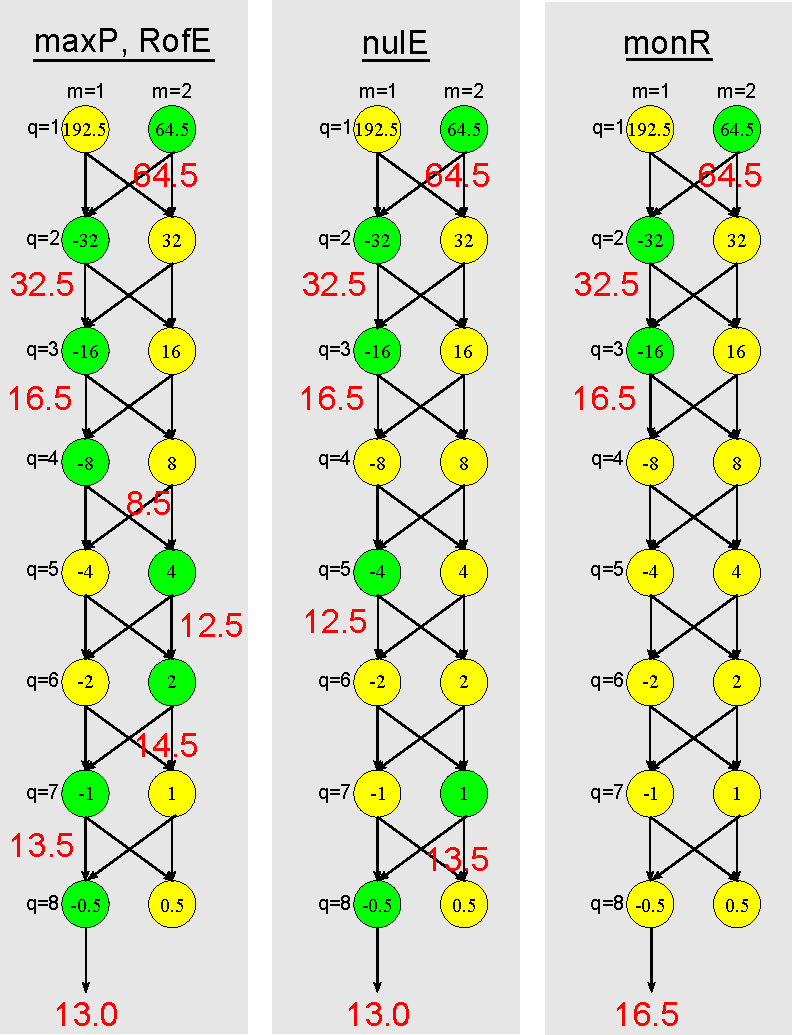
\includegraphics[height=3in]{figs/RVQ_CAC_toyExample_8x2.pdf}}
								\subfigure[Decoded outputs produced by monR.  Whereas maxP, RofE, nulE produce perfect reconstructions, monR produces quite a few incorrect reconstructions.]{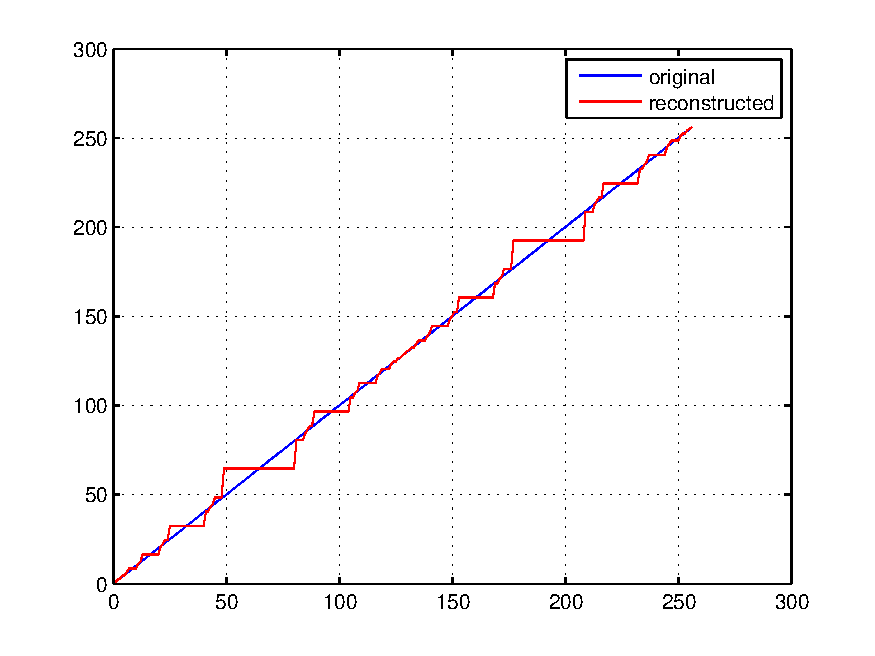
\includegraphics[height=2in]{figs/RVQ_CAC_toyExample_8x2_monR.pdf}}
								\caption{8x2 (8 stages, 2 code-vectors per stage) RVQ codebook generated with the training set, S=$\{1, 2, \ldots 256\}$.}
								\label{fig:RVQ_toy_8x2}
								\end{figure}

\begin{equation}
d_r = \dr
\end{equation}

Here, $\boldsymbol\mu_k$ is closest centroid to $\mathbf{x}_i$, $Q_i$ is the number of stages required to decode $\mathbf{x}_i$, and $\lambda$ is a regularization parameter.  With this distance measure, the likelihood of a data point being generated by an RVQ codebook $\Phi$ is given by,

\begin{equation}
p(\mathbf{x}_i|\Phi) = \frac{e^{-\big(\dr\big)}} {\sum\limits_{i=1}^N e^{-\big(\dr\big)}}
\end{equation}

%================================
\section{Experiments}
%================================
In this section, we experiment with 4 RVQ decode methods:

\begin{enumerate}
\item \underline{maxQ}: In this method, RVQ decoding is carried out so that maximum stages $Q$ are used.
\item \underline{RofE}: In this method, realm of experience coding is used.  A test vector is decoded such that the decode path traversed belongs to the set of training decode paths.
\item \underline{nulE}: In this method, null encoding is used.  Reconstruction rms error is checked at every stage.  If at any stage, rms error is not reduced, that stage is skipped until maximum stages are attained.
\item \underline{monR}: In this method, monotonic rms error is a condition.  If this condition is not met, decoding stops.
\end{enumerate}

We start with some trivial scalar examples where the training and test sets are the same.  We then move to the other extreme end of the spectrum using random data in high dimensional spaces with several observations and where the training and test sets have the same distributions but have different data.  After these experiments, we will get to tracking examples and use the likelihood formulation we have developed for RVQ.

\subsection{Scalars, S=$\{4, 6, 8, 10, 20, 22, 24, 26\}$}
%-------------------------------------------------------------
In this experiment, we train 8x2, 8x4 and 8x8 RVQ codebooks on the set of scalars, S=$\{4, 6, 8, 10, 20, 22, 24, 26\}$.  The resulting codebook for the 8x2 case is shown graphically in Figure~\ref{fig:RVQ_toy_3x2}.  In this initial experiment, the test data is the same as the training data.  Also shown in the figure is the decode path taken by the 4 methods through the RVQ trellis to to decode the number 8.  For monR, when reconstruction reaches 7 in the very first stage, rms error is 1.  However, both next stage codevectors decrease rmse which is why monR exits at this point.  All other methods are able to decode 8 correctly.  These results are shown in Table~\ref{table:results}.  
  
 
\subsection{Scalars, S=$\{1, 2, \ldots 256\}$}
%------------------------------------------------
In this experiment, we train 8x2, 8x4 and 8x8 RVQ codebooks on the set of scalars, S=$\{1, 2, \ldots 256\}$.  The resulting codebook for the 8x2 case is shown graphically in Figure~\ref{fig:RVQ_toy_8x2}.  In this initial experiment, the test data is the same as the training data.  Also shown in the figure is the decode path taken by the 4 methods through the RVQ trellis to to decode the number 13.  For monR, when reconstruction reaches 16.5, rms error is 3.5.  However, both next stage codevectors decrease rmse which is why monR exits at this point.  All other methods are able to decode 13 correctly.   These results are shown in Table~\ref{table:results}. 

\subsection{Random variables in $\mathbb{R}^{1089}$}
%------------------------------------------------
In this experiment, we train an 8x2, 8x4 and 8x8 RVQ codebook on 100 realizations of a unit-variance Gaussian random variable in $\mathbb{R}^{1089}$.  Decoding is then done on a different 100 realizations of a unit-variance Gaussian random variable in $\mathbb{R}^{1089}$.  This experiment is repeated 10 times and the results are averaged and displayed in Table~\ref{table:results}.  This experiment is then repeated for a uniform random variable.

\subsection{Images}
%------------------------------------------------
In this experiment, we use actual images from our tracking dataset.  In tracking, a bootstrapping procedure normally involves manually segmenting a target of interest and storing its $x, y, w, h, \theta$ parameters.  These parameters are then converted to an affine 6-tuple.  This 6-tuple allows warping the segmented target onto a user defined rectangular grid.  This warping has the advantage of allowing the target to have a canonical representation with standard size.  Moreover, it will be in upright position.  This can be useful in learning a basis for PCA or generating a codebook for RVQ.  For the purposes of tracking, this initial affine 6-tuple can be used to initialize a particle filter.  The particle filter then generates $N_p$ 6-tuples, and uses the same warping procedure to create $N_p$ canonical targets.  The best one according to a user defined criterion is picked and its affine parameters are then used to generate $N_p$ affine 6-tuples in the next frame and so on.  Notice that in all cases, the target snippets are generated using affine 6-tuples.

In certain cases, we may not have an affine 6-tuple, or manual segmentation may be difficult, but we may need to extract a target of interest.  In cases where running a feature detector is possible, we could extract features of interest from the target of interest.  If we can beforehand determine the position of those features in our canonical grid, then an affine mapping matrix can be computed between the feature points of interest in an image and their positions in the canonical grid.  Note that we would need to determine the positions of those features on our canonical grid only once, and then for every subsequent frame, we could run a feature detector and compute our desired  affine 6-tuple from mapping those features to the features on the canonical grid.




%================================
\section{Results}
%================================
\begin{table}
\centering
\begin{tabular}{|p{2.5in}|c|p{0.7in}|c|c|c|c|}\hline
\textbf{Dataset}							&\textbf{Codebook} &\textbf{Training rmse}	&\multicolumn{4}{|c|}{\textbf{Test rmse}} \\\hline
												& 			  			 	&								&\textbf{maxQ} 		&\textbf{RofE} 		&\textbf{nulE} 		&\textbf{monR}\\\hline
$S_{\textrm{trg}}=\{4, 6, 8, 10, 20, 22, 24, 26\}$ \newline $S_{\textrm{tst}}=S_{\textrm{trg}}$ 
                                                &8x2							&0								&0						&0							&{\color{red}0} 		&0.7071\\\hline
same                                         &8x4							&0								&0						&0							&{\color{red}0} 		&0\\\hline
same                                         &8x8							&0								&0						&0							&{\color{red}0} 		&0\\\hline\hline
S=$\{1, 2, \ldots, 256\}$  \newline $S_{\textrm{tst}}=S_{\textrm{trg}}$  				
												&8x2							&0                     		&0						&0							&{\color{red}0}		&5.2723\\\hline
same                                         &8x4							&0								&0						&0							&{\color{red}0.0726} &0.8745\\\hline
same                                         &8x8							&0								&0						&0							&{\color{red}0.0090} &0.2700\\\hline\hline

$S_{\textrm{trg}} \sim \mathcal{N}(0, 1) \in \mathbb{R}^{1089}$ 	 \newline $S_{\textrm{tst}} \sim \mathcal{N}(0, 1) \in \mathbb{R}^{1089}$, $S_{\textrm{tst}} \neq S_{\textrm{trg}}$	
		              							&8x2							&1.0420						&1.0756   	 		&1.0756    				&{\color{red}1.0708} 	&1.0723\\\hline
same as above							&8x4							&0.9899						&1.0838	   	 		&1.0838    				&{\color{red}1.0701}   &1.0713\\\hline
same as above							&8x8							&0.8892						&1.1072	   	 		&1.1068    				&{\color{red}1.0716}   &1.0720\\\hline\hline
$S_{\textrm{trg}} \sim U[0, 1] \in \mathbb{R}^{1089}$ 	 \newline $S_{\textrm{tst}} \sim U[0, 1] \in \mathbb{R}^{1089}$, $S_{\textrm{tst}} \neq S_{\textrm{trg}}$	
		              							&8x2							&0.2893						&0.3150   	 		&0.3149    				&{\color{red}0.2968}	&0.2968\\\hline
same as above							&8x4							&0.2930						&0.3485   	 		&0.3482    				&{\color{red}0.3052}    &0.3052\\\hline
same as above							&8x8							&0.3294						&0.3989   	 		&0.3987    				&{\color{red}0.3190}    &0.3190\\\hline



\end{tabular}
\caption{Training and test rmse results for different datasets for all 4 RVQ methods.}
\label{table:results}
\end{table}

We carried out experiments on two opposite ends of the spectrum. 

On the simplest side were deterministic data experiments where the training and test sets were the same.  maxP and RofE naturally did well.  monR nevertheless was unable to decode correctly in quite a few occasions and the reasons have been examined in earlier sections.  

On the extremely difficult side of things were the random data experiments with high dimensional data with several observations.  In these experiments, nulE performed the best.  The reason is that even if a subsequent stage does not decrease rms error, nulE can rely on subsequent lower energy stages to nudge down its rms error.  For the Gaussian random variable experiments, training data rms error decreased with increasing code-vectors per stage.  However, test error for maxQ and RofE increased while test error for nulE and monR did not show a clear trend.  For uniform random variable experiments, both training and test rms errors increased with number of code-vectors per stage.  It appears that whereas the uniform distribution has a clear trend, increasing error with code-vectors per stage, finding a clear trend with the gaussian random variable is more challenging.

It may be noted that the rms errors obtained were quite high for the random data sets.  The reason is quite clearly that the datasets we picked were extremely challenging.  It is expected that much better performance will be achieved with data sets in which correlations in the data can be exploited, for instance in images.

%================================
\section{Conclusions}
%================================
Over the spectrum of low and high dimensional deterministic or random data, nulE performs the best.

In the next step, we will begin experiments with images.


%%-----------------------------------------------------------------
%\newpage
%\appendix
%\section{Source code}
%\label{Sec:sourceCode}
%%-----------------------------------------------------------------
%\scriptsize
%
%\lstinputlisting[language=Matlab, caption={UTIL\_2D\_affine\_apply\_transform.m}, 		label=lst:UTIL_2D_affine_apply_transform]		{UTIL_2D_affine_apply_transform.m}

\normalsize
\bibliographystyle{ieee}
\bibliography{MyCitations}
\end{document}


%Consider Figure~\ref{fig:RVQ_toy_3x2}.  In this example, an RVQ codebook with 3 stages and 2 code-vectors per stage is designed for 8 input test points in $\mathbb{R}$.  For 2 test points 25 and 27, the reconstruction rmse (root mean squared error) is the same, i.e., 1.  However, the number of stages required is 2 and 3 respectively. In this case, it is up to the application to decide if more emphasis should be placed on If maximum stages are desired, then 27 will be picked.
%Given this overview, we now move to computation of the likelihood of a data point under RVQ. 
